% mrv-boucles.tex

%-------------------------------------------------------------------------
\section{Rappels de cours}\label{boucles:cours}
%-------------------------------------------------------------------------
\begin{enumerate}
\item Comment éviter de répéter explicitement plusieurs fois de suite la même 
	séquence d'instructions ? 
\item Comment éviter de savoir à l'avance combien de fois il faut répéter
	la séquence pour obtenir le bon résultat ? 
\end{enumerate}

De nouvelles instructions de contrôle de flux sont introduites pour répondre
à ces questions : les instructions itératives. 
On parle également de boucles, de répétitions ou encore d'itérations.
Nous distinguerons 2 variantes d'instructions itératives (Table \ref{table:python:boucles}):
l'itération conditionnelle (\texttt{while}) et le parcours de séquences (\texttt{for}).
\begin{table}[ht]
$$\begin{tabular}{|l|l|}
\hline
\multicolumn{2}{|c|}{Instructions itératives}\\
\hline
itération conditionnelle & {\begin{minipage}[t]{6cm}\tt while condition : blocWhile \\ \mbox{} \end{minipage}} \\
\hline
parcours de séquence & {\begin{minipage}[t]{7cm}\tt for element in sequence : blocFor \\ \mbox{} \end{minipage}} \\
\hline
\multicolumn{2}{p{10cm}}{où {\tt while}, {\tt for} et {\tt in} sont des mots réservés, 
{\tt condition} une expression booléenne (à valeur {\tt True} ou {\tt False}), 
{\tt element} un élément de la séquence {\tt sequence}
et {\tt bloc...} un bloc d'instructions.}
\end{tabular}$$
\caption{Instructions itératives en \python}
\label{table:python:boucles}
\end{table}

A propos des instructions itératives,
on parle souvent des boucles « {\tt while} » ou des boucles « {\tt for} » 
dans le jargon des informaticiens.

%-------------------------------------------------------------------------
\subsection{Itération conditionnelle}
%-------------------------------------------------------------------------
%$$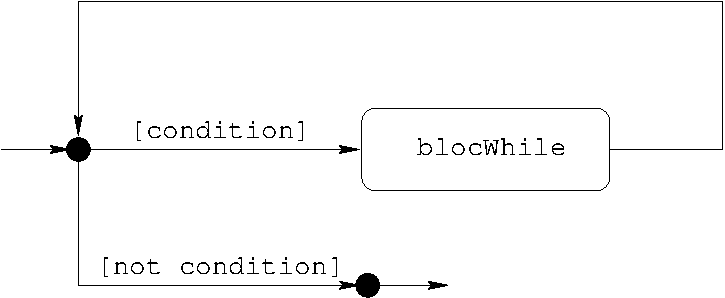
\includegraphics[width=7.5cm]{fig/uml4.pdf}$$

L'instruction « {\tt while} » permet de répéter plusieurs fois une même instruction 
(Figure \ref{figure:uml:while}) : le bloc d'instructions {\tt blocWhile} est exécuté 
tant que (\emph{while}) la condition est vérifiée. On arrête dès que la condition est fausse; 
on dit alors qu'on « sort » de la boucle. 

On commence par tester la condition; si elle
est vérifiée, on exécute le bloc d'instructions {\tt blocWhile} 
(encore appelé le «~corps~» de la boucle) puis on reteste la condition : 
la condition est ainsi évaluée avant chaque exécution du corps 
de la boucle; si la condition est à nouveau vérifiée on réexécute le bloc 
d'instructions {\tt blocWhile} (on dit qu'on « repasse » dans la boucle)
et ainsi de suite jusqu'à ce que la condition devienne fausse, 
auquel cas on « sort » de la boucle.

\begin{definition}[itération conditionnelle]
L'itération conditionnelle est une instruction de contrôle du flux d'instructions
qui permet sous condition préalable de répéter zéro ou plusieurs fois la même instruction.
\end{definition}

Dans une itération conditionnelle, la condition doit évoluer au cours des différents passages
dans la boucle afin de pouvoir sortir de la boucle. 
En ce qui concerne le nombre de passages dans la boucle, deux cas extrèmes peuvent se produire : 
\begin{itemize}
\item la condition n'est pas vérifiée la première fois : 
	on ne passe alors jamais dans la boucle.
	
	Exemple : 
	\begin{minipage}[t]{5cm}
	\begin{Verbatim}
	x = 4
	y = 0
	while x < 0 : y = y + x
	\end{Verbatim}
	\end{minipage}\hfill
	\begin{minipage}[t]{7.5cm}\footnotesize
	$x$ est positif; la condition $x < 0$ n'est donc pas vérifiée la première
	fois : on ne rentre pas dans la boucle.
	\end{minipage}
\item la condition n'est jamais fausse : on ne sort jamais de la boucle; 
	on dit qu'on a affaire à une boucle « sans fin ».

	Exemple : 
	\begin{minipage}[t]{5cm}
	\begin{Verbatim}
	x = 4
	y = 0
	while y >= 0 : y = y + x
	\end{Verbatim}
	\end{minipage}\hfill
	\begin{minipage}[t]{7.5cm}\footnotesize
	$y$ est initialement nul : on rentre dans la boucle;
	l'instruction du corps de la boucle ne peut qu'incrémenter $y$
	puisque $x$ est positif : $y$ sera donc toujours positif et on 
	ne sortira jamais de la boucle.
	\end{minipage}
\end{itemize}
Le cas de la boucle « sans fin » est évidemment dû le plus souvent à une erreur involontaire
qu'il faut savoir détecter assez vite pour éviter un programme qui « tourne » indéfiniment
sans s'arrêter.

Dans tous les cas, que l'on connaisse ou non {\em a priori} le nombre de passages dans la boucle, on peut
toujours utiliser l'itération conditionnelle (boucle {\tt while}) pour répéter plusieurs fois un bloc
d'instructions à condition de connaître la condition d'arrêt pour sortir de la boucle.
\begin{itemize}
\item Lorsqu'on connaît {\em a priori} le nombre de passages dans la boucle, 
	il suffit de définir un compteur qui compte le nombre
	de fois où on passe dans la boucle.
	On initialise correctement ce compteur avant la boucle, 
	on incrémente le compteur dans le corps de la boucle
	et on sort de la boucle lorsque ce compteur dépasse le nombre de fois connu
	où on doit passer dans la boucle.
\item Lorsqu'on ne connaît pas {\em a priori} le nombre de passages dans la boucle, 
	il faut absolument déterminer la condition d'arrêt
	de l'algorithme.
	Il faut également s'assurer que cette condition sera bien atteinte au bout d'un certain 
	nombre de passages dans la boucle.
\end{itemize}


%-------------------------------------------------------------------------
\subsection{Parcours de séquences}
%-------------------------------------------------------------------------
Il est fréquent de manipuler des suites ordonnées d'éléments comme 
les chaînes de caractères (exemple : {\tt s = "123"}), les tableaux
(exemple : {\tt t = [1,2,3]}) et les n-uplets (exemple : {\tt u = 1,2,3}).
Chaque élément d'une séquence est accessible par son rang dans la séquence 
grâce à l'opérateur « crochets » : {\tt sequence[rang]} (exemples : {\tt s[1]}, {\tt t[2]} ou {\tt u[0]}) et par convention, 
le premier élément d'une séquence a le rang {\tt 0} (exemples : {\tt s[1]} est le $2^{\grave eme}$
élément de la chaîne {\tt s}, {\tt t[2]} le $3^{\grave eme}$ élément du tableau {\tt t}
et {\tt u[0]} le $1^{er}$ élément du n-uplet {\tt u}).

\begin{minipage}[t]{4cm}
\begin{Verbatim}
>>> s = "123"
>>> s[1]
'2'
\end{Verbatim}
\end{minipage}
\hfill
\begin{minipage}[t]{4cm}
\begin{Verbatim}
>>> t = [1,2,3]
>>> t[2]
3
\end{Verbatim}
\end{minipage}
\hfill
\begin{minipage}[t]{4cm}
\begin{Verbatim}
>>> u = 1,2,3
>>> u[0]
1
\end{Verbatim}
\end{minipage}

\begin{definition}[séquence]
Une séquence est une suite ordonnée d'éléments, éventuellement vide, 
accessibles par leur rang dans la séquence.
\end{definition}

\noindent Les principales opérations sur les séquences sont listées 
dans le tableau ci-dessous
$$\begin{tabular}{|l|p{9cm}|}
\hline 
\makebox[5.5cm][l]{\bf Operation} &	\bf Result 	\\
\hline
\tt x in s      & {\tt True} if an item of {\tt s} is equal to {\tt x}, else {\tt False} \\ 	
\tt x not in s 	& {\tt False} if an item of {\tt s} is equal to {\tt x}, else {\tt True}\\
\hline 	
\tt s1 + s2 	& the concatenation of {\tt s1} and {\tt s2}\\ 	 
\tt s * n, n*s 	& {\tt n} copies of {\tt s} concatenated \\	
\hline
\hline
\tt s[i] 	& {\tt i}'th item of {\tt s}, origin {\tt 0}\\ 	
\tt s[i: j]     & \\
\tt s[i: j:step]& Slice of {\tt s} from {\tt i} (included) to {\tt j}(excluded). 
                  Optional {\tt step} value, possibly negative (default: {\tt 1}). \\	
\hline
\tt len(s) 	& Length of s \\	 
\tt min(s) 	& Smallest item of s \\	
\tt max(s) 	& Largest item of s \\
\hline
\hline
\tt range([start,] end [, step]) & Returns list of ints from {\tt >=} {\tt start} and {\tt <} {\tt end}.\newline
	With 1 arg, list from {\tt 0..arg-1}\newline
	With 2 args, list from {\tt start..end-1}\newline
	With 3 args, list from {\tt start} up to {\tt end} by {\tt step}\\
\hline
\end{tabular}$$

La dernière fonction de ce tableau crée un tableau d'entiers compris entre {\tt start} inclus
(= 0 par défaut) et {\tt end} exclus par pas de {\tt step} (= 1 par défaut).

\begin{minipage}[t]{5cm}
\begin{Verbatim}
>>> range(3)
[0, 1, 2]
>>> range(3,9,2)
[3, 5, 7]
>>> range(7,0,-1)
[7, 6, 5, 4, 3, 2, 1]
\end{Verbatim}
\end{minipage}
\hfill
\begin{minipage}[t]{5cm}
\begin{Verbatim}
>>> s = "bonjour"
>>> range(len(s))
[0, 1, 2, 3, 4, 5, 6]
>>> t = [4,2,6,5,3]
>>> range(max(t),min(t),-1)
[6, 5, 4, 3]
\end{Verbatim}
\end{minipage}
\hfill
\begin{minipage}[t]{5cm}
\begin{Verbatim}
>>> u1 = 10,12,14
>>> u2 = 'a','b','c'
>>> range(len(u1+u2))
[0, 1, 2, 3, 4, 5]
>>> range(len(2*u2[0:2]))
[0, 1, 2, 3]
\end{Verbatim}
\end{minipage}
\vspace*{1mm}

\noindent Il existe une instruction de contrôle adaptée au parcours de séquence :
$$\fbox{\tt for element in sequence : blocFor}$$
$$\begin{minipage}{6.5cm}équivalente à : 
\begin{minipage}[t]{4cm}
\begin{Verbatim}
i = 0
while i < len(s):
    element = sequence[i]
    blocFor
    i = i + 1
\end{Verbatim}
\end{minipage}
\end{minipage}$$

%-------------------------------------------------------------------------
\subsection{Imbrications de boucles}
%-------------------------------------------------------------------------
De la même manière que l'on peut cascader des alternatives simples
(voir section \ref{sub:alternatives}), on peut encapsuler une boucle 
dans une autre boucle.


Les instructions composées ont toujours la même structure : 
une ligne d'en-tête terminée par un double point ({:}), suivie
d'une ou de plusieurs instructions indentées (décalées à droite)
sous cette ligne d'en-tête (figure \ref{fig:bloc}).

\begin{minipage}[t]{5cm}
\begin{Verbatim}
ligne d'en-tête:
    première instruction du bloc
    ...
    dernière instruction du bloc
\end{Verbatim}
\end{minipage}

\noindent S'il y a plusieurs instructions indentées sous la ligne d'en-tête, elles doivent l'être exactement au
même niveau (décalage de 4 caractères espace, par exemple). Ces instructions indentées
constituent ce qu'on appellera désormais un bloc d'instructions. Un bloc d'instructions est une
suite d'instructions formant un ensemble logique, qui n'est exécuté que dans certaines conditions
définies dans la ligne d'en-tête. Dans l'exemple précédent, les deux lignes
d'instructions indentées sous la ligne contenant l'instruction « {\tt while i < 10:} » constituent un même 
bloc logique : ces deux lignes ne sont exécutées -- toutes les deux -- que si la condition testée 
avec l'instruction {\tt while} est vérifiée, c'est-à-dire si le multiplicateur {\tt i}
est tel que {\tt 1 <= i < 10}.


%-------------------------------------------------------------------------
\subsection{Exécutions de boucles}
%-------------------------------------------------------------------------
La maîtrise de l'algorithmique requiert deux qualités complémentaires \cite{darmengeat} :
\begin{itemize}
\item il faut avoir une certaine intuition, car aucun algorithme ne permet de 
	savoir {\em a priori} quelles instructions permettront d'obtenir le résultat 
	recherché. C'est là qu'intervient la forme « d'intelligence » 
	requise pour l'algorithmique : la « créativité » de l'informaticien. 
	Il y a des gens qui possèdent au 
	départ davantage cette intuition que les autres.  
	Cependant, les réflexes, cela s'acquiert (en particulier, l'annexe \ref{invariant}
	page \pageref{invariant} présente une méthode pour aider à construire des boucles). 
	Et ce qu'on appelle l'intuition n'est finalement que de l'expérience accumulée,
	tellement répétée que le raisonnement, au départ laborieux, finit par 
	devenir «~spontané~».
\item il faut être méthodique et rigoureux. En effet, chaque fois qu'on écrit 
	une série d'instructions que l'on croit justes, il faut systématiquement 
	se mettre mentalement à la place de la machine qui va les exécuter
	(sur papier ou dans sa tête) afin de vérifier si le résultat obtenu 
	est bien celui que l'on voulait. 
	Cette opération ne requiert pas d'intuition. Mais elle reste néanmoins indispensable
	si l'on ne veut pas écrire des algorithmes à l'« aveuglette ».
	Et petit à petit, à force de pratique, on fera
	de plus en plus souvent l'économie de cette dernière étape : 
	l'expérience fera qu'on « verra » le résultat produit par les instructions, 
	au fur et à mesure qu'on les écrira. 
	Naturellement, cet apprentissage est long, et demande des heures de 
	travail patient. 
	Aussi, dans un premier temps, il faut éviter de sauter les étapes : la vérification méthodique, 
	pas à pas, de chacun des algorithmes représente plus de la moitié du travail à accomplir\ldots
	et le gage de progrès.
\end{itemize}

Pour améliorer la compréhension d'une boucle, on peut « tracer » son exécution de tête,
à la main ou par programme. Dans tous les cas, l'idée est de suivre pas à pas
l'évolution des variables qui interviennent dans la boucle : on détermine leur valeur 
juste avant la boucle, à la fin de chaque itération et juste après la boucle.

%-------------------------------------------------------------------------
\subsection{Construction d'une boucle}
%-------------------------------------------------------------------------
Un algorithme est un mécanisme qui fait passer un « système » d'une « situation »
dite initiale (ou précondition) à une « situation » finale (postcondition ou but). 
Le couple (situation initiale, situation finale) est appelé spécification de l'algorithme. 
L'algorithmique vise donc à construire rationnellement des algorithmes à partir de 
leur spécification.

Le raisonnement qui permet de passer d'une compréhension intuitive d'un
tel énoncé à l'algorithme n'est pas toujours facile à concevoir d'un coup. 
Dans le cas d'une boucle on pourra systématiser la conception de l'algorithme
autour de 4 étapes (d'après \cite{didier} et \cite{guyomard}):
\begin{enumerate}
\item {\bf Invariant} (ou hypothèse de récurrence) : « Le clou est planté dans la planche ».
\item {\bf Condition d'arrêt} : « La tête touche la planche ».
\item {\bf Progression} : « Frapper un coup de marteau de façon à enfoncer un peu plus le clou ».
\item {\bf Initialisation} : « Planter légèrement le clou à la main ».
\end{enumerate}
Il faut noter que les étapes 1 et 2 définissent des situations
tandis que les étapes 3 et 4 concernent des actions. 
Dans cette section, on notera les situations entre crochets ({\tt []}) pour les distinguer
des actions.
\begin{itemize}
\item La recherche d'un invariant est l'étape clé autour de laquelle s'articule la conception des boucles. 
	La conjonction de l'invariant et de la condition d'arrêt conduit logiquement au but recherché :
	$$\fbox{\begin{minipage}{13cm}\tt
	[« invariant » and « condition d'arrêt »] $\Rightarrow$ [« postcondition »]
	\end{minipage}}$$
	La condition d'arrêt seule n'implique pas le but.

\item La progression doit :
	\begin{itemize}
	\item conserver l'invariant.
		Plus précisément, la progression est un fragment d'algorithme
		défini par les situations initiale et finale suivantes :\\
		\mbox{}\hspace*{5mm}situation initiale : {\tt [« invariant » and not « condition d'arrêt »]}\\
		\mbox{}\hspace*{5mm}situation finale : {\tt [« invariant »]}\\ 
		$$\fbox{\begin{minipage}{13cm}\tt
		\mbox{}[« invariant » and not « condition d'arrêt »]\\
		\mbox{}« progression »\\
		\mbox{}[« invariant »]
		\end{minipage}}$$
	\item faire effectivement progresser vers le but pour faire en sorte que la condition 
		d'arrêt soit atteinte au bout d'un temps fini.
	\end{itemize}
\item  L'initialisation doit instaurer l'invariant. 
	Plus précisément, elle doit, partant de la précondi\-tion, atteindre l'invariant.
		$$\fbox{\begin{minipage}{13cm}\tt
		\mbox{}[« précondition »]\\
		\mbox{}« initialisation »\\
		\mbox{}[« invariant »]
		\end{minipage}}$$

\end{itemize}
D'une manière plus générale, les 4 étapes de construction d'une boucle
sont les suivantes :
\begin{enumerate}
\item {\bf Invariant :} proposer une situation générale décrivant le problème posé (hypothèse de
	récurrence). C'est cette étape qui est la plus délicate car elle exige de faire 
	preuve d'imagination.

\item {\bf Condition d'arrêt :} à partir de la situation générale imaginée en [1], on doit
	formuler la condition qui permet d'affirmer que l'algorithme a terminé son travail. 
	La situation dans laquelle il se trouve alors est appelée situation finale.
	La condition d'arrêt fait sortir de la boucle.

\item {\bf Progression :} se « rapprocher » de la situation finale, tout en faisant le nécessaire pour
	conserver à chaque étape une situation générale analogue à celle retenue en [1].
	La progression conserve l'invariant.
	
\item {\bf Initialisation :} initialiser les variables introduites dans l'invariant 
	pour que celui-ci soit vérifié avant d'entrer dans la boucle.
	L'initialisation « instaure » l'invariant.
	
\item {\bf Boucle finale :} Une fois les 4 étapes précédentes menées à leur terme, l'algorithme recherché 
	aura la structure finale suivante (figure \ref{fig:invariant}) :
	$$\begin{minipage}[t]{4cm}
	\begin{verbatim}
	[« précondition »]
	« initialisation »
	[« invariant »]
	while not [« condition d'arrêt »] :
	    « progression »
	    [« invariant »]
	[« postcondition »]
	\end{verbatim}
	\end{minipage}$$
	Quand on sort de la boucle, la situation finale attendue est atteinte.
	
	Dans la pratique, on ne garde que les instructions :
	$$\fbox{\begin{minipage}[t]{8cm}\tt
	« initialisation »\\
	while [not « condition d'arrêt »] : \\
	\mbox{}\ \ \ \ « progression »
	\end{minipage}}$$
	\begin{minipage}[t]{6cm}
	Exemple de la puissance \ref{ex:puissance} :\\
	{\tt k = 1}\\
	{\tt p = x}\\
	{\tt while not k > n: }\\
	{\tt \mbox{}\ \ \ \ p = p*x}\\
	{\tt \mbox{}\ \ \ \ k = k + 1}
	\end{minipage}
	\hfill
	\begin{minipage}[t]{6cm}
	Exemple du pgcd \ref{ex:pgcd3} :\\
	{\tt while not b == 0:}\\
	{\tt \mbox{}\ \ \ \ r = a\%b}\\
	{\tt \mbox{}\ \ \ \ a = b}\\
	{\tt \mbox{}\ \ \ \ b = r}
	\end{minipage}
	
	Un des problèmes, pour l'apprenti informaticien, est que la boucle finale
	ainsi obtenue ne fait pas apparaître explicitement l'invariant dans le code. 
	L'invariant est une aide conceptuelle pour construire la boucle, 
	mais pas pour l'exécuter.
\end{enumerate}

\begin{definition}
Un invariant de boucle est une propriété vérifiée tout au long de 
l'exécution de la boucle. 
\end{definition}

Cette façon de procéder permet de « prouver » la validité de l'algorithme au fur et à
mesure de son élaboration. En effet la situation générale choisie en [1] est en fait l'invariant 
qui caractérise la boucle {\tt while}.
Cette situation est satisfaite au départ grâce à l'initialisation de l'étape [4]; 
elle reste vraie à chaque itération (étape [3]). Ainsi lorsque la condition d'arrêt (étape [2])
est atteinte cette situation nous permet d'affirmer que le problème est résolu.
C'est également en analysant l'étape [3] qu'on peut prouver la terminaison de l'algorithme.


%-------------------------------------------------------------------------
\section{Vie courante : }\label{boucles:vie-courante}
%-------------------------------------------------------------------------

\subsection{Objectif}\label{boucles:vie-courante:objectif}
\begin{description}
\item[Principal : ] mettre en \oe uvre une instruction d'itération.
\item[Secondaire :] .
\end{description}


\subsection{Syntaxe \python}\label{boucles:vie-courante:python}

\subsection{Enoncé}\label{boucles:vie-courante:enonce}

\subsection{Méthode}\label{boucles:vie-courante:methode}

\subsection{Résultat}\label{boucles:vie-courante:resultat}

\subsection{Vérification}\label{boucles:vie-courante:verification}

\subsection{Généricité}\label{boucles:vie-courante:genericite}

\subsection{Entraînement}\label{boucles:vie-courante:entrainement}

%-------------------------------------------------------------------------
\section{Jeux : }\label{boucles:jeux}
%-------------------------------------------------------------------------

\subsection{Objectif}\label{boucles:jeux:objectif}
\begin{description}
\item[Principal : ] mettre en \oe uvre une instruction d'itération.
\item[Secondaire :] .
\end{description}

\subsection{Syntaxe \python}\label{boucles:jeux:python}

\subsection{Enoncé}\label{boucles:jeux:enonce}

\subsection{Méthode}\label{boucles:jeux:methode}

\subsection{Résultat}\label{boucles:jeux:resultat}

\subsection{Vérification}\label{boucles:jeux:verification}

\subsection{Généricité}\label{boucles:jeux:genericite}

\subsection{Entraînement}\label{boucles:jeux:entrainement}


%-------------------------------------------------------------------------
\section{Textes : compter les voyelles}\label{boucles:textes}
%-------------------------------------------------------------------------

\subsection{Objectif}\label{boucles:textes:objectif}
\begin{description}
\item[Principal : ] mettre en \oe uvre une instruction d'itération.
\item[Secondaire :] compter le nombre de voyelles dans une chaîne de caractères.
\end{description}

\subsection{Syntaxe \python}\label{boucles:textes:python}

\subsection{Enoncé}\label{boucles:textes:enonce}

\subsection{Méthode}\label{boucles:textes:methode}

\subsection{Résultat}\label{boucles:textes:resultat}

\subsection{Vérification}\label{boucles:textes:verification}

\subsection{Généricité}\label{boucles:textes:genericite}

\subsection{Entraînement}\label{boucles:textes:entrainement}

%-------------------------------------------------------------------------
\section{Nombres : conversion décimal $\rightarrow$ binaire}\label{boucles:nombres}
%-------------------------------------------------------------------------

\subsection{Objectif}\label{boucles:nombres:objectif}
\begin{description}
\item[Principal : ] mettre en \oe uvre une instruction d'itération.
\item[Secondaire :] convertir un entier décimal en un entier binaire.
\end{description}

\subsection{Syntaxe \python}\label{boucles:nombres:python}

\subsection{Enoncé}\label{boucles:nombres:enonce}

\subsection{Méthode}\label{boucles:nombres:methode}

\subsection{Résultat}\label{boucles:nombres:resultat}

\subsection{Vérification}\label{boucles:nombres:verification}

\subsection{Généricité}\label{boucles:nombres:genericite}

\subsection{Entraînement}\label{boucles:nombres:entrainement}

%-------------------------------------------------------------------------
\section{Figures : tracé d'un heptagone régulier}\label{boucles:figures}
%-------------------------------------------------------------------------

\subsection{Objectif}\label{boucles:figures:objectif}
\begin{description}
\item[Principal : ] mettre en \oe uvre une instruction d'itération.
\item[Secondaire :] tracer un heptagone régulier.
\end{description}

\subsection{Syntaxe \python}\label{boucles:figures:python}

\subsection{Enoncé}\label{boucles:figures:enonce}

\subsection{Méthode}\label{boucles:figures:methode}

\subsection{Résultat}\label{boucles:figures:resultat}

\subsection{Vérification}\label{boucles:figures:verification}

\subsection{Généricité}\label{boucles:figures:genericite}

\subsection{Entraînement}\label{boucles:figures:entrainement}

%-------------------------------------------------------------------------
\section{Mathématiques : intégration de $\cos(x)$}\label{boucles:maths}
%-------------------------------------------------------------------------

\subsection{Objectif}\label{boucles:maths:objectif}
\begin{description}
\item[Principal : ] mettre en \oe uvre une instruction d'itération.
\item[Secondaire :] calculer l'intégrale de la fonction cosinus.
\end{description}

\subsection{Syntaxe \python}\label{boucles:maths:python}

\subsection{Enoncé}\label{boucles:maths:enonce}

\subsection{Méthode}\label{boucles:maths:methode}

\subsection{Résultat}\label{boucles:maths:resultat}

\subsection{Vérification}\label{boucles:maths:verification}

\subsection{Généricité}\label{boucles:maths:genericite}

\subsection{Entraînement}\label{boucles:maths:entrainement}

%-------------------------------------------------------------------------
\section{Physique : sorties d'un circuit logique}\label{boucles:physique}
%-------------------------------------------------------------------------

\subsection{Objectif}\label{boucles:physique:objectif}
\begin{description}
\item[Principal : ] mettre en \oe uvre une instruction d'itération.
\item[Secondaire :] déterminer la table de vérité d'un circuit logique.
\end{description}

\subsection{Syntaxe \python}\label{boucles:physique:python}

\subsection{Enoncé}\label{boucles:physique:enonce}

\subsection{Méthode}\label{boucles:physique:methode}

\subsection{Résultat}\label{boucles:physique:resultat}

\subsection{Vérification}\label{boucles:physique:verification}

\subsection{Généricité}\label{boucles:physique:genericite}

\subsection{Entraînement}\label{boucles:physique:entrainement}

%-------------------------------------------------------------------------
\section{Informatique : }\label{boucles:informatique}
%-------------------------------------------------------------------------

\subsection{Objectif}\label{boucles:informatique:objectif}
\begin{description}
\item[Principal : ] mettre en \oe uvre l'instruction d'itération.
\item[Secondaire :] .
\end{description}

\subsection{Syntaxe \python}\label{boucles:informatique:python}

\subsection{Enoncé}\label{boucles:informatique:enonce}

\subsection{Méthode}\label{boucles:informatique:methode}

\subsection{Résultat}\label{boucles:informatique:resultat}

\subsection{Vérification}\label{boucles:informatique:verification}

\subsection{Généricité}\label{boucles:informatique:genericite}

\subsection{Entraînement}\label{boucles:informatique:entrainement}


%-------------------------------------------------------------------------
\section{Retours d'expériences}\label{boucles:retours}
%-------------------------------------------------------------------------

%-------------------------------------------------------------------------
\subsection{Méthode}\label{boucles:retours:methode}

%-------------------------------------------------------------------------
\subsection{Résultat}\label{boucles:retours:resultat}

%-------------------------------------------------------------------------
\subsection{Vérification}\label{boucles:retours:verification}

